\documentclass[hyperref={breaklinks,colorlinks,
   urlcolor=blue,citecolor=blue,linkcolor=red}]{beamer}
   %\setbeamercolor{section in head/foot}{bg=black}
   

\definecolor{PHSmagenta}{cmyk}{0.45,0.85,0,0}
\definecolor{PHSpurple}{cmyk}{0.85,0.9,0,0}
\definecolor{PHSblue}{cmyk}{0.80,0.25,0,0}
\definecolor{PHSgreen}{cmyk}{0.55,0,1,0}
\definecolor{PHSgraphite}{cmyk}{0.25,0.25,0,0.4}
\definecolor{PHSteal}{cmyk}{0.85,0.30,0.5,0.15}
\definecolor{PHSliberty}{cmyk}{0.5,0.5,0,0.4}
\definecolor{PHSrust}{cmyk}{0.2,0.85,1,0.1}

\definecolor{GUblue}{RGB}{0, 0, 140} %b204,b153
\definecolor{mayablue}{rgb}{0.45, 0.76, 0.98}
\definecolor{lightcornflowerblue}{rgb}{0.6, 0.81, 0.93}
%\usecolortheme[named=PHSmagenta]{structure}

\setbeamercolor{section in head/foot}{bg=PHSpurple} % Top/bottom with section and page number

\setbeamercolor{structure}{fg=PHSpurple}%Title, top subsection bar, section

\setbeamercolor{subsection in head/foot}{bg=PHSpurple} % subsection bar

\setbeamercolor{author in head/foot}{bg=PHSpurple}%bottom with name and institute


\mode<presentation>
{
  \usetheme{Ilmenau} %Madrid, AnnArbor, Goettingen, Warsaw,CambridgeUS
  %\usecolortheme{seahorse} %whale, beaver,rose,crane, wolverine
  \usefonttheme{serif}
  
  
}
\makeatletter 
\beamer@theme@subsectionfalse%
\makeatother

\setbeamertemplate{frametitle continuation}{}

\newcommand{\backupbegin}{
   \newcounter{finalframe}
   \setcounter{finalframe}{\value{framenumber}}
}
\newcommand{\backupend}{
   \setcounter{framenumber}{\value{finalframe}}
}

\usepackage[round]{natbib}
\usepackage{amsmath}
\usepackage{graphicx}
\usepackage{verbatim}
\usepackage[english]{babel}
\usepackage[absolute,overlay]{textpos}
\usepackage{caption}
\captionsetup{font=scriptsize}
\usepackage{amssymb}
\usepackage{tcolorbox}
\usepackage{tipa}
\usepackage{booktabs}
\usepackage{siunitx}
\usepackage{adjustbox}
\usepackage{setspace}
\usepackage{lipsum}
\usepackage{physics}
\usepackage{qrcode}
\renewcommand{\vec}[1]{\boldsymbol{#1}}
\newcommand{\Hmns}{\tiny\textrm{H}}
\usepackage{media9}
\usepackage{aasmacros}
\usepackage{multimedia}
\usepackage{sidecap}
\usepackage{tikz}
\usetikzlibrary{arrows,positioning}
\usepackage{xcolor}
\usepackage{listings}

\definecolor{codegreen}{rgb}{0,0.6,0}
\definecolor{codegray}{rgb}{0.5,0.5,0.5}
\definecolor{codepurple}{rgb}{0.58,0,0.82}
\definecolor{backcolour}{rgb}{0.95,0.95,0.92}

\lstdefinestyle{mystyle}{
    backgroundcolor=\color{backcolour},   
    commentstyle=\color{codegreen},
    keywordstyle=\color{magenta},
    numberstyle=\tiny\color{codegray},
    stringstyle=\color{codepurple},
    basicstyle=\ttfamily\footnotesize,
    breakatwhitespace=false,         
    breaklines=true,                 
    captionpos=b,                    
    keepspaces=true,                 
    numbers=left,                    
    numbersep=5pt,                  
    showspaces=false,                
    showstringspaces=false,
    showtabs=false,                  
    tabsize=2
}

\lstset{style=mystyle}



\setbeamertemplate{caption}[numbered]{\centering\raggedright}


\newcommand\FourQuad[4]{%
    \begin{minipage}[b][.35\textheight][t]{.47\textwidth}#1\end{minipage}\hfill%
    \begin{minipage}[b][.35\textheight][t]{.47\textwidth}#2\end{minipage}\\[0.5em]
    \begin{minipage}[b][.35\textheight][t]{.47\textwidth}#3\end{minipage}\hfill
    \begin{minipage}[b][.35\textheight][t]{.47\textwidth}#4\end{minipage}%
}


\usepackage{xspace}
\newcommand{\bilby}{{\sc Bilby}\xspace}
\newcommand{\PyCBC}{{\sc PyCBC}\xspace}
\newcommand{\IPython}{{\sc IPython}\xspace}
\newcommand{\Python}{{\sc Python}\xspace}
\newcommand{\Numpy}{{\sc NumPy}\xspace}
\newcommand{\astropy}{{\sc Astropy}\xspace}
\newcommand{\gwpy}{{\sc GWpy}\xspace}
\newcommand{\lal}{{\sc LALSimulation}\xspace}



\usepackage{etoolbox}

\makeatletter

% Patch case where name and year are separated by aysep
\patchcmd{\NAT@citex}
  {\@citea\NAT@hyper@{%
     \NAT@nmfmt{\NAT@nm}%
     \hyper@natlinkbreak{\NAT@aysep\NAT@spacechar}{\@citeb\@extra@b@citeb}%
     \NAT@date}}
  {\@citea\NAT@nmfmt{\NAT@nm}%
   \NAT@aysep\NAT@spacechar\NAT@hyper@{\NAT@date}}{}{}

% Patch case where name and year are separated by opening bracket
\patchcmd{\NAT@citex}
  {\@citea\NAT@hyper@{%
     \NAT@nmfmt{\NAT@nm}%
     \hyper@natlinkbreak{\NAT@spacechar\NAT@@open\if*#1*\else#1\NAT@spacechar\fi}%
       {\@citeb\@extra@b@citeb}%
     \NAT@date}}
  {\@citea\NAT@nmfmt{\NAT@nm}%
   \NAT@spacechar\NAT@@open\if*#1*\else#1\NAT@spacechar\fi\NAT@hyper@{\NAT@date}}
  {}{}

\makeatother

\defbeamertemplate*{footline}{myminiframes theme}
  {%
    \begin{beamercolorbox}[colsep=1.5pt]{upper separation line foot}
    \end{beamercolorbox}
    \begin{beamercolorbox}[ht=2.5ex,dp=1.125ex,%
      leftskip=.3cm,rightskip=.3cm plus1fil]{author in head/foot}%
      \leavevmode{\usebeamerfont{author in head/foot}\insertshortauthor}%
      \hfill%
      {\usebeamerfont{institute in head/foot}\usebeamercolor[fg]{institute in head/foot}\insertshortinstitute}%
    \end{beamercolorbox}%
    \begin{beamercolorbox}[ht=2.5ex,dp=1.125ex,%
      leftskip=.3cm,rightskip=.3cm plus1fil]{title in head/foot}%
      {\usebeamerfont{title in head/foot}\insertshorttitle\hfill \insertframenumber/\inserttotalframenumber}%<-here
    \end{beamercolorbox}%
    \begin{beamercolorbox}[colsep=1.5pt]{lower separation line foot}
    \end{beamercolorbox}
  }
\makeatother

\addtobeamertemplate{headline}{\hypersetup{linkcolor=.}}{}
\addtobeamertemplate{footline}{\hypersetup{linkcolor=.}}{}
%\setbeamertemplate{author in head/foot}{}

\beamertemplatenavigationsymbolsempty

\title[Hierarchical Geography]
{Hierarchical Geography with \Python}
\subtitle{A Very Brief Introduction}
\author[Gerald Leung]{Gerald Leung\inst{1}} %\\ Supervisor: Ik Siong Heng\inst{1}}
\institute[PHS Geospatial]{\inst{1}Public Health Scotland\\
\texttt{gerald.leung@phs.scot}}%{\inst{1}School of Physics and Astronomy,\\ University of Glasgow}
\date[\today]{\today}
\logo{
\includegraphics[scale=0.03]{PHS logo positive}}
\titlegraphic{
\includegraphics[scale=0.055]{PHS logo positive}}


%\logo{\includegraphics[scale=0.8]{SchPhyAst_colour.png}}

\begin{document}

{
\setbeamertemplate{logo}{}
\begin{frame}
\titlepage
%\vspace{-2cm}
%\begin{center}
%\includegraphics[width=0.40\textwidth]{SchPhyAst_colour.png}\includegraphics[width=0.30\textwidth]{cu_logo_4c_centre-eps-converted-to.pdf}
%\end{center}
\end{frame}
}



\section{Introduction}

\begin{frame}{Background}
\begin{itemize}
\item{We use GP boundaries as an example}
\begin{itemize}
\item{areas covered are defined with different geographies}
\item{e.g. postcode districts and sectors}
\item{ultimately we are only interested in the overall boundary of a GP}
\end{itemize}
\item{How do we merge geographies at different levels?}
$\Longrightarrow \textrm{\texttt{GeoPandas} in \Python}$
\item{You can find the \IPython Notebook \href{https://github.com/Gerald-Leung/GP_Boundaries/blob/main/Geographies\%20.ipynb}{here} on GitHub}
\end{itemize}
\end{frame}

\section{\texttt{GeoPandas}}
\begin{frame}{\texttt{GeoPandas}}
\begin{itemize}
\item{An open source project for geospatial data analysis in \Python~\citep{kelsey_jordahl_2020_3946761}}
\item{Extends from \texttt{Pandas}~\citep{pandas},
a data analysis package}
\item{Can be used to read and create shape files}
\end{itemize}
%\begin{figure}
%\begin{center}
%\includegraphics[scale=0.55]{total}
%\caption{All admission statistics for patients aged 65 or above. An increasing trend could be observed.}
%\end{center}
%\end{figure}
\end{frame}

\section{Data}
\begin{frame}{NRS Data}
We make use of postcode district
and sector data from the National Records of Scotland (\href{https://www.nrscotland.gov.uk/statistics-and-data/geography/nrs-postcode-extract}{NRS}).
\begin{itemize}
\item{Shape files}
\item{Contain geometries of districts and sectors}
\item{Read in as \texttt{DataFrames} into \Python with
\texttt{Pandas}}
\item{Convert to \texttt{GeoDataFrames} with \texttt{GeoPandas}}
\end{itemize}
\end{frame}

\begin{frame}{NRS Data}
\begin{figure}
\begin{center}
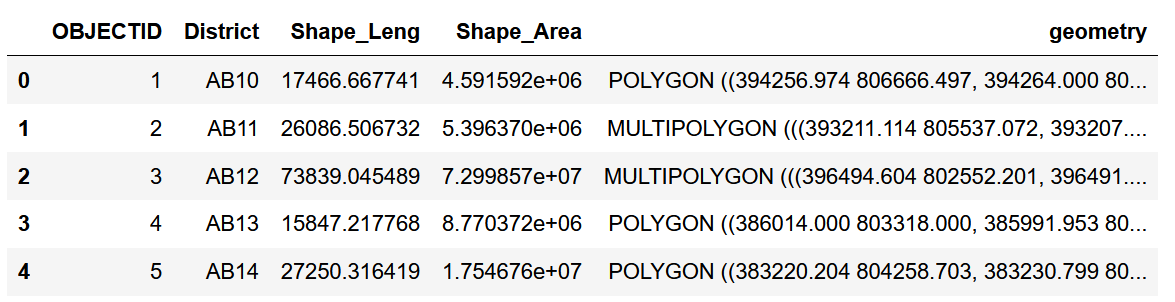
\includegraphics[scale=0.5]{districtcolumns}
\caption{A segment of \texttt{DataFrame} containing district information. Similarly for sector data, with a column
representing postcode sectors.}
\end{center}
\end{figure}
\end{frame}

\begin{frame}{GP Data}
\begin{itemize}
\item{For this example we make use of a few GPs from Lanarkshire (with some modifications):}
\begin{itemize}
\item{Nalagatla Medical Practice}
\item{The Craigallian Avenue Practice}
\item{The Stonelaw Practice}
\item{Ardoch Medical Practice}
\end{itemize}
\end{itemize}
\end{frame}

\begin{frame}{Hypothetical GP}
\begin{itemize}
\item{For the purpose of testing, we also create two hypothetical practices, namely Hypothetical One and Hypothetical Two respectively}
\begin{itemize}
\item{They cover areas defined by a combination of districts and sectors}
\end{itemize}
\end{itemize}
\end{frame}

\begin{frame}{Data Wrangling}
Steps are taken to make sure that
the data are presented consistently:
\begin{itemize}
\item{Separate the comma separated areas of the GPs into
individual rows}
\item{Distinguish and separate districts and sectors into different columns}
\end{itemize}
\end{frame}

\begin{frame}{Data Wrangling}
%\newgeometry{left=10mm,right=80mm}
\begin{columns}
\begin{column}{\dimexpr\paperwidth-10pt}
\begin{table}
\begin{center}
\begin{tabular}{c | c | c}
\toprule
\texttt{Practice Code} & \texttt{Practice Name} & \texttt{Areas} \\
\midrule
\midrule
\vdots & \vdots & \vdots\\
\texttt{66667} & \texttt{Hypothetical Two} & \texttt{G68,G74 4}\\ 
\bottomrule
\end{tabular}
\caption{An example of how the dataset would look like \textbf{before} data wrangling.}
\end{center}
\end{table}
\end{column}
\end{columns}
%\restoregeometry
\end{frame}

\begin{frame}{Data Wrangling}
%\newgeometry{left=10mm,right=80mm}
\begin{columns}
\begin{column}{\dimexpr\paperwidth-10pt}
\begin{table}
\begin{center}
\begin{tabular}{c | c | c |c}
\toprule
\texttt{Practice Code} & \texttt{Practice Name} & \texttt{District} & \texttt{Sector} \\
\midrule
\midrule
\texttt{60073} & \texttt{Nalagatla Medical Practice} & \texttt{NaN} & \texttt{G33 6}\\
%60177 & The Craigallian Avenue Practice & \texttt{NaN} & \texttt{G72 7}\\
\vdots & \vdots & \vdots & \vdots\\
\texttt{60092} & \texttt{The Stonelaw Practice} & \texttt{G76} & \texttt{NaN}\\
\texttt{66667} & \texttt{Hypothetical Two} & \texttt{NaN} & \texttt{G74 4}\\
\texttt{66667} & \texttt{Hypothetical Two} & \texttt{G68} & \texttt{NaN}\\ 
\bottomrule
\end{tabular}
\caption{An example of how the dataset would look like \textbf{after} data wrangling.}
\end{center}
\end{table}
\end{column}
\end{columns}
%\restoregeometry
\end{frame}

\begin{frame}[fragile]{Joining the Data}
Now that we have our GP (\texttt{hyposplit}) and NRS data (\texttt{sectors} and \texttt{districts}), we merge them together.
First merge sector data:
\begin{lstlisting}[language=Python,frame=single]
# Firstly merge with sector data to get their
# geometries and remove irrelevant rows
merged = pd.merge(hyposplit,sectors,on="Sector",how="outer")   
merged = merged.head(39)                                      
\end{lstlisting}
\end{frame}

\begin{frame}[fragile]{Joining the Data}
Then we merge our district data:
\begin{lstlisting}[language=Python,frame=single]
# Now merge with district data for their geometries 
# Again we keep only rows with our GP data
merged = pd.merge(merged,districts,on="District",how="outer")  
merged = merged.head(39)                                       
\end{lstlisting}
\end{frame}

\begin{frame}[fragile]{Convert to \texttt{GeoDataFrame}}
For a \texttt{DataFrame DF}, we can easily convert it to a
\texttt{GeoDataFrame GDF} with
\begin{lstlisting}[language=Python,frame=single]
import geopandas as gpd
GDF = gpd.GeoDataFrame(DF, crs="EPSG:4326")
\end{lstlisting}
where \texttt{EPSG:4326} refers to the current
coordinate system (latitude and longitude) based on the Earth's centre of mass.
\end{frame}

\section{Results}
\begin{frame}{Undissolved Boundaries}
\begin{columns}
\begin{column}{0.5\textwidth}
\begin{itemize}
\item{First plot the initial results in \texttt{Matplotlib}
as a sanity check}
\item{Some boundaries may not be visible due to overlapping}
\item{Notice the boundaries are `undissolved' - we can still see different levels (sectors and districts) of geographies}
\end{itemize}
\end{column}

\begin{column}{0.7\textwidth}
\begin{figure}
\begin{center}
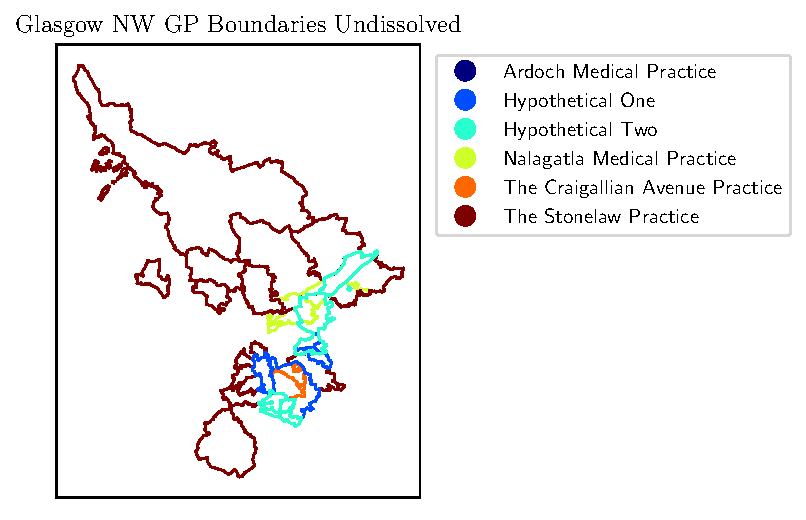
\includegraphics[scale=0.5]{geography_test}
\caption{Undissolved Glasgow NW GP boundaries.}
\end{center}
\end{figure}
\end{column}
\end{columns}
\end{frame}

\begin{frame}[fragile]{Merging Geographies}
\begin{columns}
\begin{column}{0.5\textwidth}
\begin{itemize}
\item{We are interested in the overall boundaries of the GPs}
\item{Need to merge the individual postcode districts and sectors of a GP}
\item{We can dissolve the boundaries and merge the geographies}
\end{itemize}
\end{column}

\begin{column}{0.6\textwidth}
For undissolved \texttt{GeoDataFrame uGDF}, we can simply dissolve the geographies by grouping and merging the \texttt{Practice Code} column:
\begin{lstlisting}[language=Python,frame=single]
dissolved = uGDF.dissolve(by="Practice Code")
\end{lstlisting} 
\end{column}
\end{columns}
\end{frame}

\begin{frame}{Dissolved Boundaries}
We plot the final results again as a sanity check:
\begin{figure}
\begin{center}
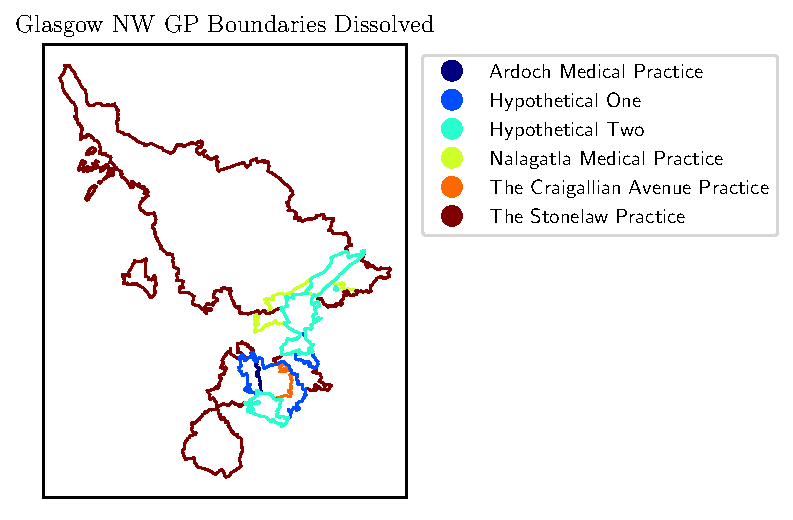
\includegraphics[scale=0.6]{geography_dissolved}
\caption{Dissolved Glasgow NW GP boundaries.}
\end{center}
\end{figure}
\end{frame}

\begin{frame}{Mapping on \texttt{ArcGIS}}
\begin{figure}
\begin{center}
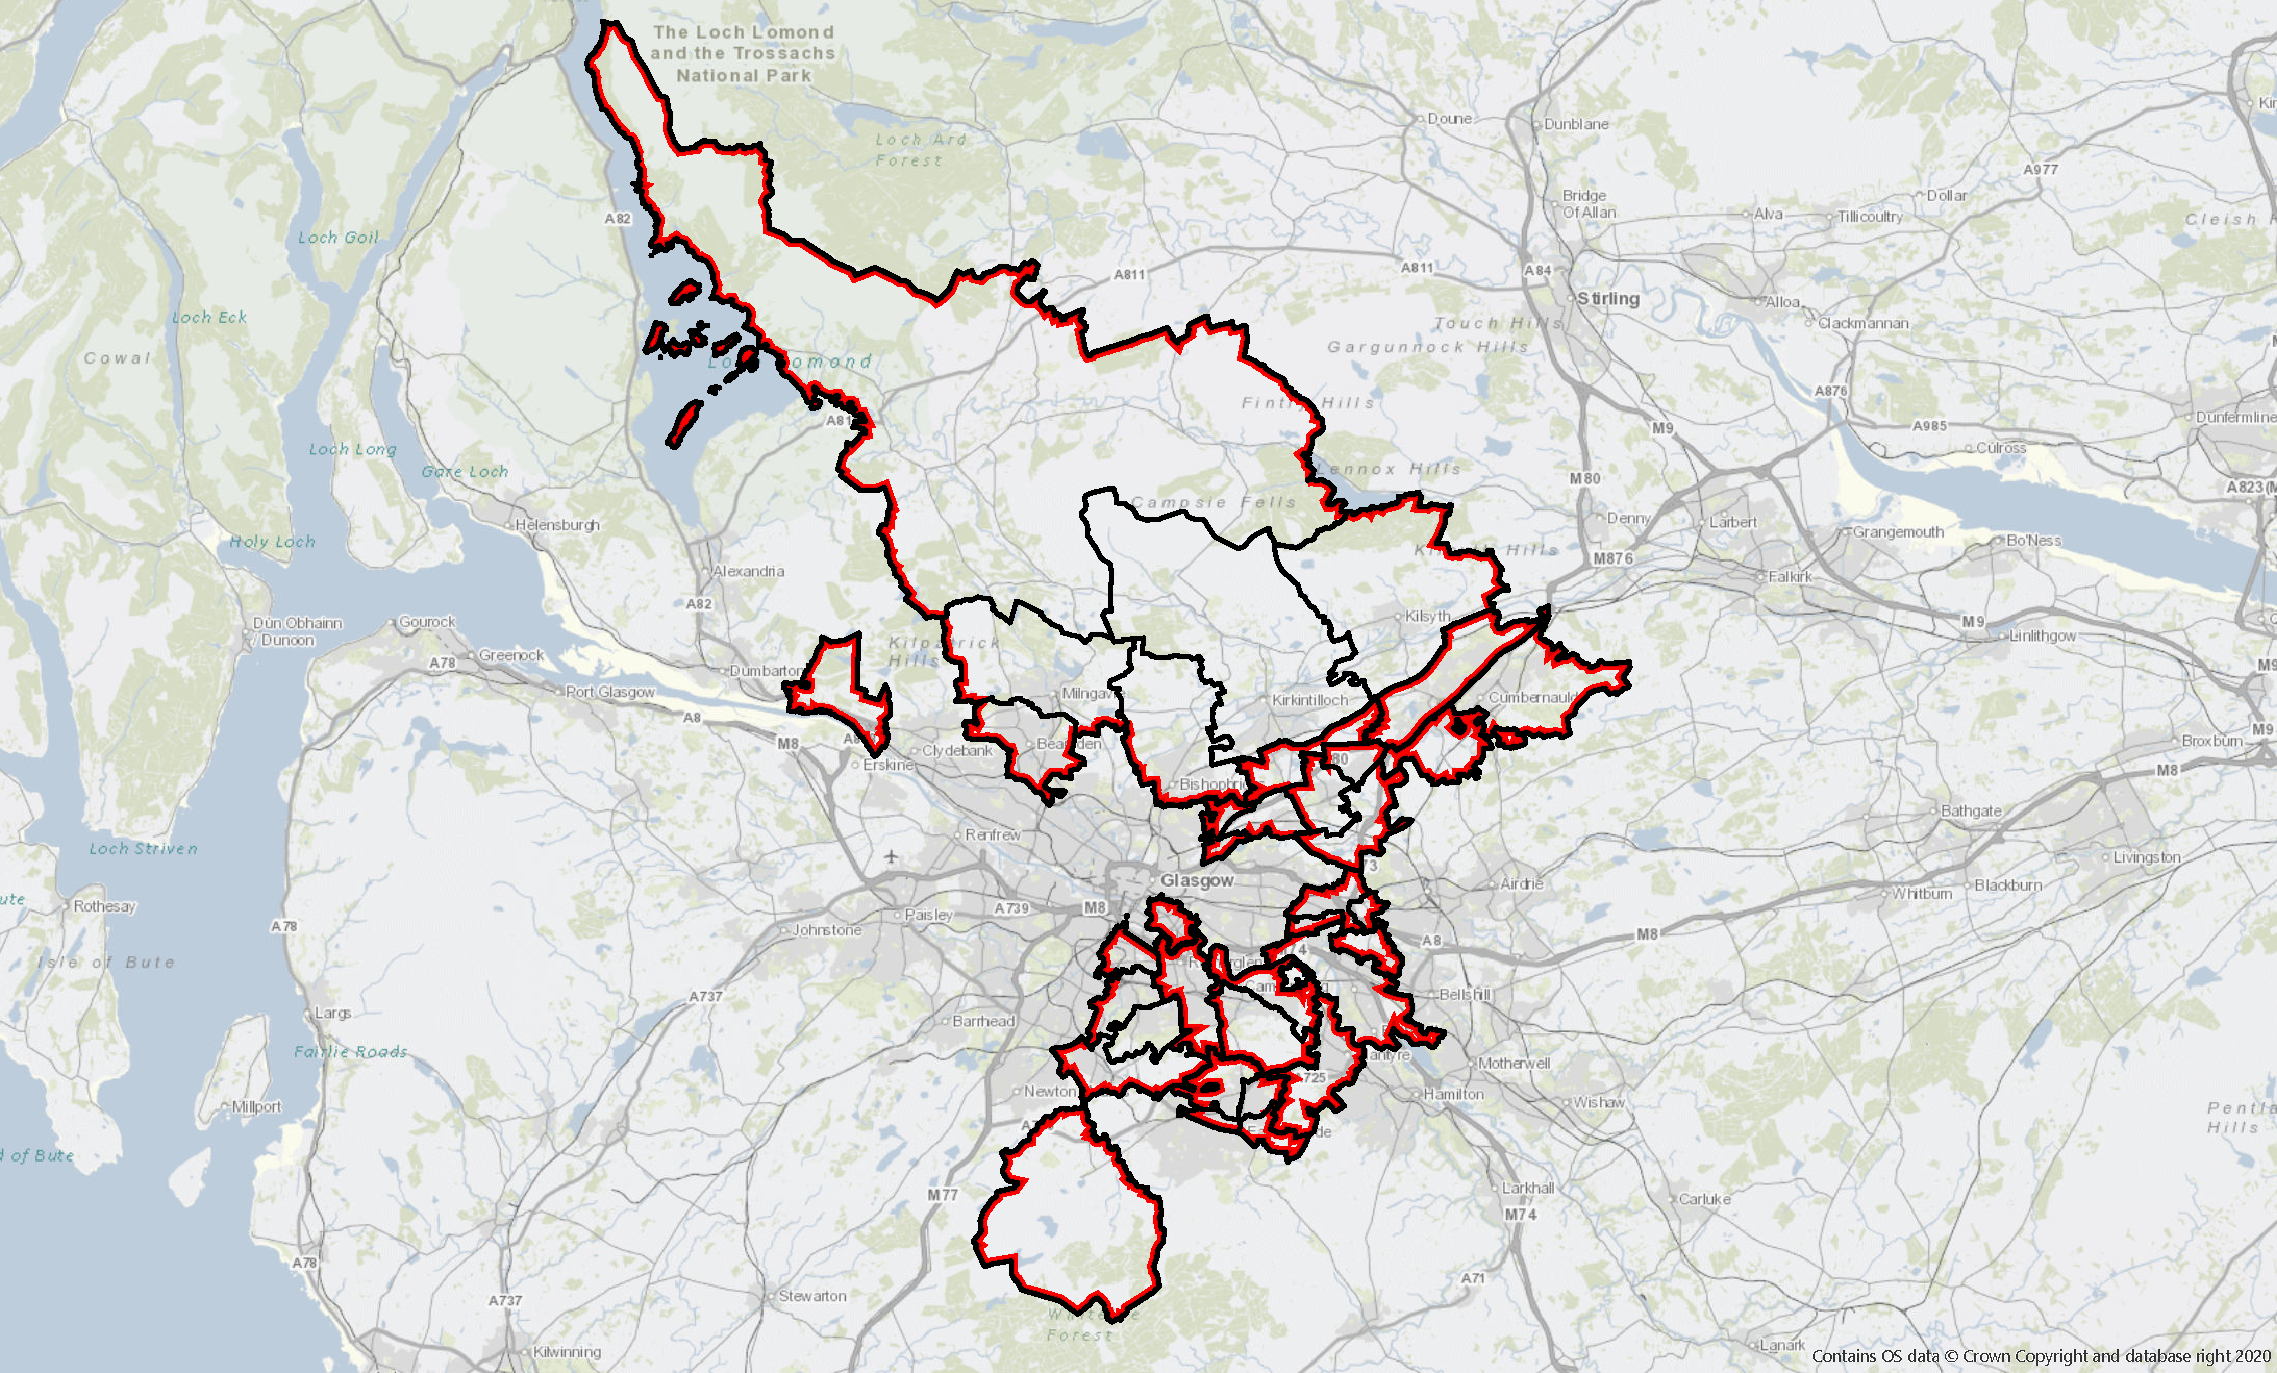
\includegraphics[scale=0.23]{Map.pdf}
\caption{Glasgow NW GP boundaries. Black lines
represent all geography levels (sectors and districts). Red lines represent the overall boundaries of a GP (with geographies disolved).}
\end{center}
\end{figure}
\end{frame}

\section{Conclusion}
\begin{frame}{Summary}
\begin{itemize}
\item{\texttt{Pandas} and \texttt{GeoPandas} in \Python
provide simple methods to deal with shape files}
\item{Can apply to other scenarios where we have to deal with a hierarchy of geography}
\item{It takes only a few lines of codes in \Python
for this task so it is relatively simple}
\item{This is however only possible when we are provided with
numerical description (e.g. in postcode sectors/districts) of the GP boundaries}
\begin{itemize}
\item{if we are given a description by words, we will probably have to define the boundaries manually on \texttt{ArcGIS}}
\end{itemize}
\item{Naturally, this task can also be done in \texttt{ArcGIS}}
\end{itemize}

\end{frame}





%\iffalse
\begin{frame}[allowframebreaks]{References} 

%\bibliographystyle{unsrt}
%\bibliographystyle{apalike}

%\bibliographystyle{aasjournal}

%\bibliographstyle{aa_url}
\bibliographystyle{yahapj}

\bibliography{slidescites}
\end{frame}
%\fi

\end{document}
